\RequirePackage[orthodox]{nag}
\documentclass[11pt]{article}

%% Define the include path
\makeatletter
\providecommand*{\input@path}{}
\g@addto@macro\input@path{{include/}{../include/}}
\makeatother

\usepackage{../../include/akazachk}

\title{ECH4905 ChemE Optimization HW 1}
\author{Andres Espinosa}

\begin{document}
\maketitle

\section{Problem 1}
Consider the following matrix and perform the following calculations showing all your steps.
\begin{align*}
    A = 
  \begin{bmatrix}
     2 & 2 & 3 \\
     1 & -1 &0 \\
     -1 & 2 &1
  \end{bmatrix}
\end{align*}
\subsection{Part a}
Determinant of A
\begin{gather*}
    \det A = 
    2 (-1(1) - 0) - 2(1(1) + 0) + 3((1)(2) - (-1)(-1)) \\
    = -2 -2 + 6 - 3 \\
    \det A = -1
\end{gather*}

\subsection{Part b}
Eigenvalues and eigenvectors of A
\begin{gather*}
    (2- \lambda) ((-1 - \lambda)(1 - \lambda) - 0) - 2(1(1- \lambda) + 0) + 3((1)(2) - (-1-\lambda)(-1)) = 0 \\
    -(2-\lambda)(1+\lambda)(1-\lambda) -2(1-\lambda) + 6 -3(1+\lambda) = 0 \\
    -(2-\lambda)(1+\lambda)(1-\lambda) + (1-\lambda) \\
    (1-\lambda)((1+\lambda)(\lambda-2)+1) \\
    (1-\lambda)(\lambda^2 - \lambda -2 +1) \\
    (1-\lambda)(\lambda^2 - \lambda -1) \\
    \lambda = 1, \frac{1+\sqrt{5}}{2}, \frac{1 - \sqrt{5}}{2}
\end{gather*}

% Still need to do eigenvectors

\section{Problem 2}

\section{Problem 3}
Consider the following function and perform the following calculations
\begin{equation*}
    f(x_1, x_2) = x_1^3 x_2 - x_1 x_2^3
\end{equation*}

\subsection{Part a}
Gradient of the function
\begin{align*}
    \nabla f(x_1, x_2) = 
  \begin{bmatrix}
     3x_1^2 x_2 - x_2^3 \\
     x_1^3 - 3x_1 x_2^2
  \end{bmatrix}
\end{align*}

\subsection{Part b}
Hessian of the function
\begin{align*}
    \nabla^2 f(x_1, x_2) = 
  \begin{bmatrix}
     6x_1 x_2 & 3x_1^2 - 3x_2^2 \\
     3x_1^2 - 3x_2^2 &  6 x_1 x_2
  \end{bmatrix}
\end{align*}

\subsection{Part c}
Write the second order Taylor expansions around a point $(x_1^*, x_2^*)$
%Still need to do this

\section{Problem 4}

\section{Problem 5}

\section{Problem 6}

\section{Problem 7}
Consider the following optimization problem
\begin{align}
  \text{minimize} & \quad x_1 \\
  \text{subject to} & \quad x_1 + x_2 \leq 10 \\
  & \quad x_1 - 2x_2 \geq 1 \\
  & \quad x_1, x_2 \geq 0 \\
  & \quad x_1, x_2 \in \mathbb{R}
\end{align}

\subsection{Part a}
This problem is an LP. The constraints are all linear and the variables are continuous variables in $\mathbb{R}$.

\subsection{Part b}

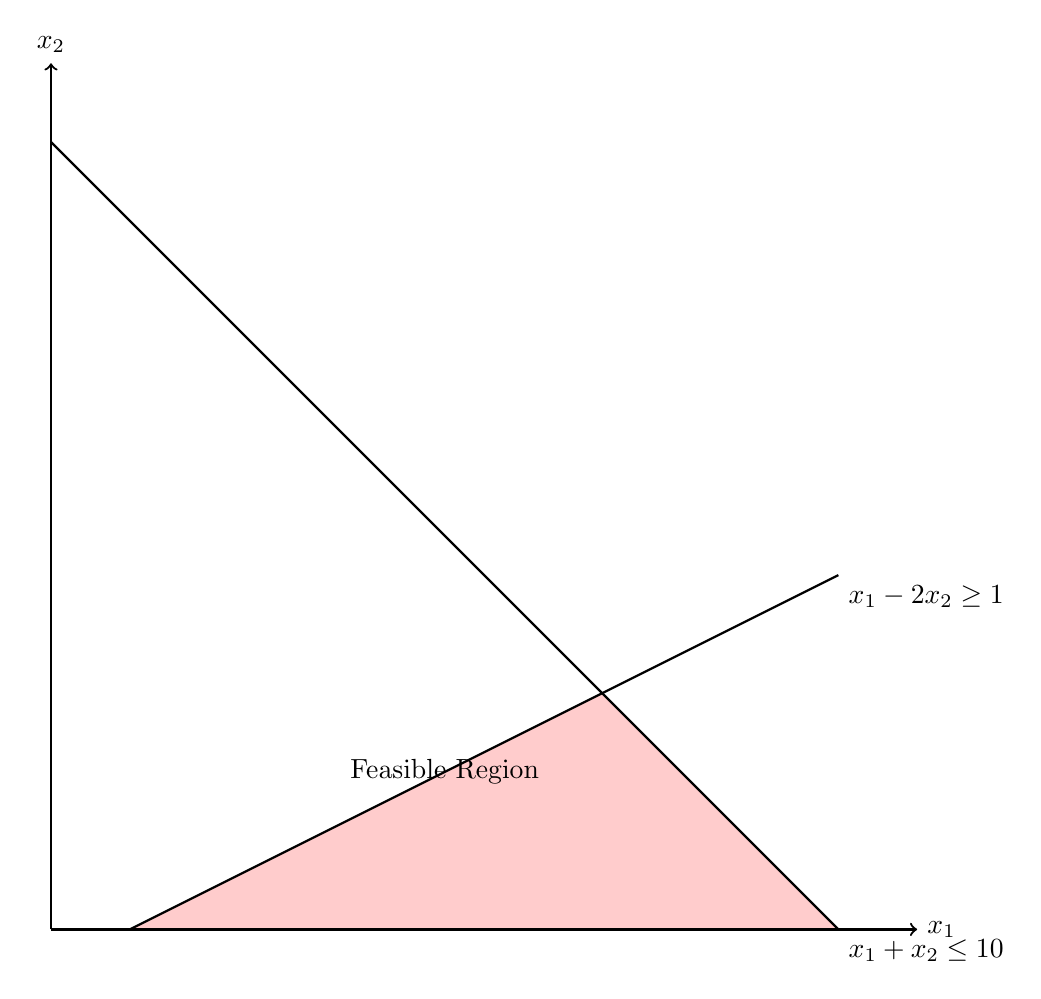
\begin{tikzpicture}
    \fill[red!20] (1,0) -- (10,0) -- (5,5) -- (7,3) -- cycle;
    \draw[thick, ->] (0,0) -- (11,0) node[right] {$x_1$};
    \draw[thick, ->] (0,0) -- (0,11) node[above] {$x_2$};
    \draw[thick] (0,10) -- (10,0) node[below right] {$x_1 + x_2 \leq 10$};
    \draw[thick] (1,0) -- (10,4.5) node[below right] {$x_1 - 2x_2 \geq 1$};
    \node at (5,2) {Feasible Region};
\end{tikzpicture}

\subsection{Part c}

The problem is convex. 
The objective function is convex as it is linear. 
The feasible region is also convex because it is the intersection of half-spaces.
The feasible region is a polyhedron.

\section{Problem 8}Consider the following optimization problem
\begin{align}
  \text{minimize} & \quad x_1 \\
  \text{subject to} & \quad x_1 + x_2 \leq 10 \\
  & \quad x_1 - 2x_2 \geq 1 \\
  & \quad x_1, x_2 \geq 0 \\
  & \quad x_1, x_2 \in \mathbb{R}
\end{align}

\subsection{Part a}
This problem is a MILP. 
The constraints and objective function are all linear and the variables are binary integer variables.
Therefore it is not a standard LP, but instead an MILP.

\subsection{Part b}

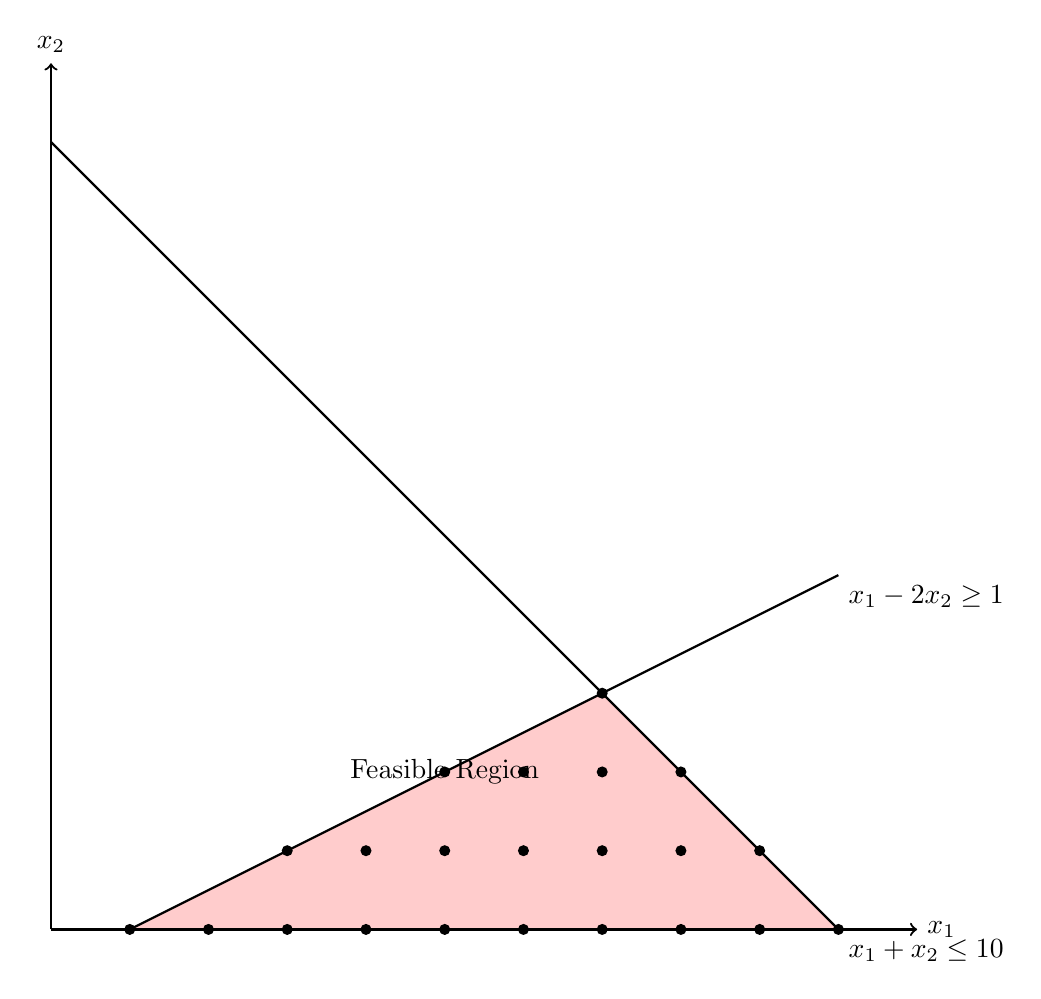
\begin{tikzpicture}
    % Shaded feasible region - keep as is to show the feasible region
    \fill[red!20] (1,0) -- (10,0) -- (5,5) -- (7,3) -- cycle;

    % Axes
    \draw[thick, ->] (0,0) -- (11,0) node[right] {$x_1$};
    \draw[thick, ->] (0,0) -- (0,11) node[above] {$x_2$};

    % Constraints
    \draw[thick] (0,10) -- (10,0) node[below right] {$x_1 + x_2 \leq 10$};
    \draw[thick] (1,0) -- (10,4.5) node[below right] {$x_1 - 2x_2 \geq 1$};

    % Feasible region label
    \node at (5,2) {Feasible Region};

    % Manually mark specific points
    \def\markpoint(#1,#2){
                \fill (#1,#2) circle (2pt);
    }

    % Mark several points manually
    \markpoint(1,0)
    \markpoint(2,0)
    \markpoint(3,0)
    \markpoint(4,0)
    \markpoint(5,0)
    \markpoint(6,0)
    \markpoint(7,0)
    \markpoint(8,0)
    \markpoint(9,0)
    \markpoint(10,0)
    \markpoint(3,1)
    \markpoint(4,1)
    \markpoint(5,1)
    \markpoint(6,1)
    \markpoint(7,1)
    \markpoint(8,1)
    \markpoint(9,1)


    \markpoint(5,2)
    \markpoint(6,2)
    \markpoint(7,2)
    \markpoint(8,2)
  
 
    \markpoint(7,3)
   



\end{tikzpicture}

\subsection{Part c}

The problem is non-convex because there are integer variables. 
The disjoint that integer variables introduce naturally make the problem non-convex.


\end{document}